\problemset{Статистический анализ}
\problemset{Индивидуальное домашнее задание №2}

\renewcommand*{\proofname}{Решение}
\textbf{Часть 1}

В результате эксперимента получены данные. \\

\begin{tabular}{|c|c|c|c|c|c|c|c|c|c|c|c|c|c|c|c|c|c|c|c|c|c|c|c|c|}
	\hline
	0&1&1&1&1&0&0&0&2&0&1&0&0&1&1&1&2&0&0&0&0&4&0&1&0\\ \hline 0&0&0&0&0&1&1&1&2&3&1&0&1&0&0&2&0&0&0&1&1&1&0&1&2\\
	\hline 
\end{tabular}
\\

\begin{tabular}{|c|c|c|c|c|}
	\hline
	$\alpha_1=0.10$ & $a = 0.00$ & $b = 1.37$ & $\lambda_0=0.70$ & $\lambda_1=1.40$ \\
	\hline
\end{tabular}


\begin{problem}
	Построить вариационный ряд, эмпирическую функцию распределения и гистограмму частот.
\end{problem}

\begin{proof}
	$ $
		
	Вариационный ряд:
	
	0 0 0 0 0 0 0 0 0 0 0 0 0 0 0 0 0 0 0 0 0 0 0 0 0 1 1 1 1 1 1 1 1 1 1 1 1 1 1 1 1 1 1 2 2 2 2 2 3 4 
	
	Построим таблицу частот для выборки. \\
		
	\begin{tabular}{|c|c|c|c|c|c|}
		\hline
		$x_j$&0&1&2&3&4\\ \hline
		$m_j$&25&18&5&1&1\\ \hline
		$p_j^*$&\frc12&\frc9{25}&\frc1{10}&\frc1{50}&\frc1{50} \\
		\hline
	\end{tabular}
	\\
	
	Построим эмпирическую функцию распределения по полученным данным:\\
	
	 $F(x)=\left\{ 
	\begin{gathered} 
		0, x \leqslant 0 \hfill \\  
		0.5, 0 < x \leqslant 1 \hfill \\
		0.86, 1 < x \leqslant 2 \hfill \\
		0.96, 2 < x \leqslant 3 \hfill \\
		0.98, 3 < x \leqslant 4 \hfill \\
		1, x > 4 \hfill \\
	\end{gathered}
	\right.$	
	\begin{figure}[h]
		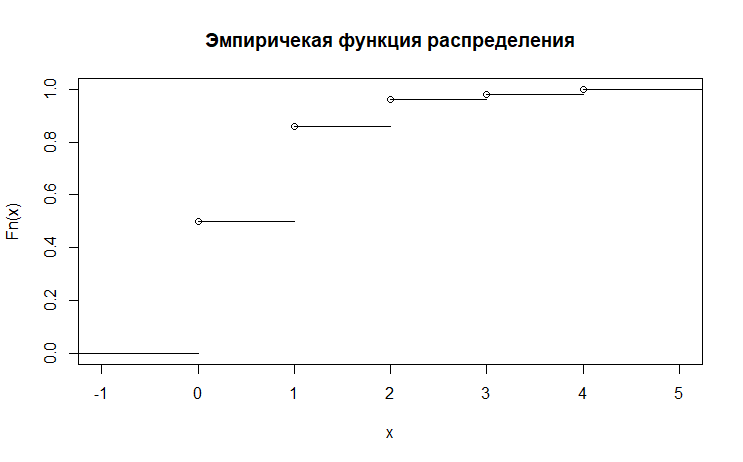
\includegraphics[scale=0.76]{Emp.png}
		\caption{Эмпирическая функция распределения}
	\end{figure}
	\begin{figure}[h]
		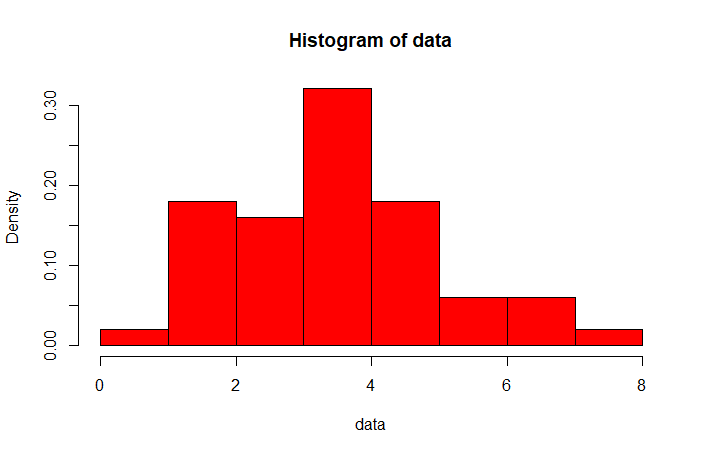
\includegraphics[scale=0.76]{Hist.png}
		\caption{Гистограмма частот}
	\end{figure}
\end{proof}


\newpage
\begin{problem}
	Вычислить выборочные аналоги следующих характеристик:
	\begin{itemize}
		\item математического ожидания
		\item дисперсии
		\item медианы
		\item ассиметрии
		\item эксцесса
		\item вероятности $P(X\in[a, b])$
	\end{itemize}
\end{problem}

\begin{proof}
	$ $
	
	\begin{itemize}
	\item Математическое ожидание:
		\begin{equation}	
		\bar x_{\text{в}} = \cfrac1n 		\sum^{n}_{i=1}x_im_i=\cfrac1{50}\cdot(18+10+7)=\cfrac{35}{50}=0.7
		\end{equation}
	\item Дисперсия:
	\begin{equation}	
		D_{\text{в}} = \bar{x^2}-\bar{x}^2=\cfrac1n\sum(x_i-\bar{x})^2=\cfrac1{50}\cdot(18+20+9+16)-0.49=\cfrac{63}{50}-0.49=1.26-0.49=0.77
	\end{equation}
	\item Медиана:
	\begin{equation}
		Me = 0.5
	\end{equation}	
	\item Ассиметрия:
	\begin{equation}
		As = \cfrac{\mu_3^*}{\sigma^3} = 1.464547
	\end{equation}
	\item Эксцесс:
	\begin{equation}
		Ex = \cfrac{\mu_4^*}{\sigma^4}-3 = 2.633496
	\end{equation}
	\item Вероятность:
	\begin{equation}
		P(x \in [a, b]) = P(x \in [0.00, 1.37]) = F(1.37) - F(0.00) = 0.86 
	\end{equation}
	\end{itemize}			
\end{proof}


\begin{problem}
	В предположении, что исходные наблюдения являются выборкой из распределения Пуассона, построить оценку максимального правдоподобия параметра $\lambda$, а также оценку $\lambda$ по методу моментов. Найти смещение оценок 	
\end{problem}

\begin{proof}
	$ $ 
	
	Распределение Пуассона:
	$P_{\lambda} = (x = k) = \cfrac{\lambda^k}{k!}\cdot \exp(-\lambda)$
	\begin{itemize}
		\item Метод максимального правдоподобия
		\begin{multline}
			l(x, \lambda) =  \cfrac{\lambda^{\sum\limits^n_1x_i}\cdot \exp (-\lambda n)}{\prod\limits_1^n x_i!}\Rightarrow ll(\bar{x}, \lambda) = \sum\limits_1^nx_iln\lambda-n\lambda-\sum\limits_1^nlnx_i!\Rightarrow \cfrac{\partial ll(\bar x, \lambda)}{\partial \lambda} = \cfrac1{\lambda}\sum\limits_1^nx_i-n=0\Rightarrow \\ \Rightarrow \hat{\lambda}= \cfrac{1}{n}\sum\limits_1^nx_i=\bar{x_{\text{в}}}=0.7
		\end{multline}
		\item Метод моментов
		\begin{align}
			&P(x, \theta) \\
			&M_1^* = \bar{x_{\text{в}}}; \mathbb{E}X = \bar{x_{\text{в}}}; \\
			&\mathbb{E}X = \int_{\mathbb{R}}xp(x, \theta)dx = \varphi(\theta) \\
			&M_1 = \mathbb{E}X=\lambda; M_1^* = \bar{x_{\text{в}}} \Rightarrow \underline{\hat{\lambda} = \bar{x_{\text{в}}} = 0.7}
		\end{align}
	\end{itemize}
	Чтобы найти смещение оценки, найдем:
	\begin{equation}
		\mathbb{E}\hat{\lambda}=\cfrac1n\sum\limits_1^n\mathbb{E}x_i=\cfrac{n\lambda}n=\lambda\Rightarrow\text{оценки несмещенные}
	\end{equation}
\end{proof}


\begin{problem}
	Построить асимптотический доверительный интервал уровня значимости $\alpha_1$ для параметра $\lambda$ на базе оценки максимального правдоподобия.	
\end{problem}

\begin{proof}
	\begin{align}
		&\hat{\lambda}=\bar{x_{\text{в}}}=0.7; \alpha_1=0.10; \gamma=1-\alpha_1=0.90; \\
		&\cfrac{\sqrt{n}(\bar{x}-\lambda)}{\sqrt{\lambda}}\underset{n\to\infty}{\longrightarrow}N(0,1) \\
		&t_\gamma: \phi(t_\gamma)=1-\cfrac{\alpha_1}2\Rightarrow t_\gamma=1.645 \\
		&P(-t_\gamma \leqslant \cfrac{\sqrt{n}(\bar{x_\text{в}}-\lambda)}{\sqrt{\lambda}} \leqslant t_\gamma)\longrightarrow 1-\alpha \\
	    &n(\bar{x_\text{в}}-\lambda)^2=t_\gamma^2\lambda \\
		&\lambda^2-2\lambda(\bar{x_\text{в}}+\cfrac{t_\gamma^2}{2n})+\bar{x_\text{в}}=0 \\
	\end{align}	
	\begin{align}
	D &= \cfrac{t_\gamma^2}{n}(\bar{x_\text{в}}+\cfrac{t_\gamma^2}{4n}) \\
	\lambda_{1,2}=\bar{x_\text{в}}+\cfrac{t_\gamma^2}{2n}\pm t_\gamma\sqrt{\cfrac1n(\bar{x_\text{в}}+\cfrac{t_\gamma^2}{4n})}&=0.7+0.027\pm0.1965\Rightarrow [0.5305; 0.9235]
\end{align}
\end{proof}


\begin{problem}
	Используя гистограмму частот, построить критерий значимости $\chi^2$ проверки простой гипотезы согласия с распределением Пуассона с параметром $\lambda_0$. Проверить гипотезу на уровне значимости $\alpha_1$. Вычислить наибольшее значение уровня значимости, на котором еще нет оснований отвергнуть данную гипотезу. 
\end{problem}

\begin{proof}
	\begin{align}
		&\hat{\lambda_0}=0.70; \alpha_1=0.10; \\
		&m_i-\text{эмпирические частоты}; \\
		&m_i^{'}-\text{выравнивающие частоты}; m_i^{'}=n\cdot p_i \\
		&\text{Простая гипотеза } H_0 \text{ имеет вид:} \\
		&H_0:p(x)=\cfrac{\lambda_0^x}{x!}\exp(-\lambda_0) \\
		&\text{Тогда искомая вероятность примет вид:} \\
		&p_k=P(X=k)=\cfrac{0.7^k}{k!}\exp(-0.7) \\
	\end{align}	

	Построим таблицу оценки методом $\chi^2$. \\
	
	\begin{tabular}{|c|c|c|c|c|c|c|}
		\hline
		$x_i$ & $0$ & $1$ & $2$ & $3$ & $4$ & $\sum$ \\ \hline 
		$m_i$ & $25$ & $18$ & $5$ & $1$ & $1$ & $50$ \\ \hline 
		$p_i$ & $0.497$ & $0.348$ & $0.122$ & $0.029$ & $0.005$ & $1$ \\ \hline 
		$m_i^{'}$ & $24.8292652$ & $17.3804856$ & $6.0831700$ & $1.4194063$ & $0.2876729$ & $50$ \\ \hline 
		$m_i-m_i^{'}$ & $0.1707348$ & $0.6195144$ & $-1.0831700$ & $-0.4194063$ & $0.7123271$ & $0$ \\ \hline 
		$\cfrac{(m_i-m_i^{'})^2}{m_i^{'}}$ & $0.001174033$ & $0.022082125$ & $0.192869374$ & $0.123926224$ & $1.763843457$ & $\chi^2_{\text{набл}}$ \\
		\hline
	\end{tabular} 

	\begin{align}
		&\chi^2_{\text{набл}}=\sum\limits_1^k\cfrac{(m_i-m_i^{'})^2}{m_i^{'}}=2.103895 \\ 
		&l=k-r-1=5-1-1=3 \\
		&\chi^2_{\text{кр}}=\chi^2_{\alpha;l} = \chi^2_3 \text{ на уровне значимости 0.1 = 6.251} \\
	\end{align}
	$\chi^2_{\text{набл}} < \chi^2_{\text{кр}}\Rightarrow$ гипотеза $H_0$ принимается, выборка принадлежит распределению Пуассона.\\
	Наибольшее значение уровня значимости, при котором еще нет оснований отвернуть данную гипотезу = $0.5511251$	
\end{proof}


\begin{problem}
	Построить критерий значимости $\chi^2$ проверки сложной гипотезы согласия с распределением Пуассона. Проверить гипотезу на уровне значимости $\alpha_1$. Вычислить наибольшее значение уровня значимости, на котором еще нет оснований отвергнуть данную гипотезу. 
\end{problem}

\begin{proof}
	$ $
	
	Сложная гипотеза $H_0$ имеет вид:
	\begin{align}
		H_0: x_1,...,x_n \sim P_{ois}(\lambda) \\
		\sum\limits_1^k\cfrac{(m_i-np_i(\lambda))^2}{np_i(\lambda)}\longrightarrow\chi^2_{k-r-1}
	\end{align}	

	Метод минимизации хи-квадрат:
	\begin{equation}
		\underset{\lambda}{argmin}\sum\limits_1^r\cfrac{(m_i-np_i(\lambda))^2}{np_i(\lambda)}
	\end{equation}
	
	Задача реализована в R следующим скриптом: \\
	
	$\begin{gathered}
		P <- function(a)\{ \hfill \\
		p <- 0 \hfill \\
		p[1] <- ppois(0, a) \hfill \\
		p[2] <- ppois(1, a) - sum(p) \hfill \\
		p[3] <- ppois(2, a) - sum(p) \hfill \\
		p[4] <- ppois(3, a) - sum(p) \hfill \\
	\end{gathered}$
	
	$\begin{gathered}
	p[5] <- 1-sum(p) \hfill \\
	p\} \hfill \\
	X2 <- function(a)\{g <- n\cdot P(a); f <- (nu-g)^2/g; sum(f)\} \hfill \\
	nu <- c(25, 17, 6, 1, 1) \hfill \\
	XM <- nlm(X2, 0.70) \hfill \\
	\end{gathered}$ \\
	
	В результате вычислений получим, что $\chi^2_{\text{набл}}=1.861649<\chi^2_{\text{крит}}=4.60517$ 
	Таким образом, гипотеза принимается. 
	
	Наибольшее значение уровня значимости, при котором еще нет оснований отвернуть данную гипотезу = $0.3942285$	
\end{proof}


\begin{problem}
	Построить наиболее мощный критерий проверки простой гипотезы пуассоновости с параметром $\lambda=\lambda_0=0.70$ при альтернативе пуассоновости с параметром $\lambda=\lambda_1=1.40$. Проверить гипотезу на уровне значимости $\alpha_1$. Что получится, если поменять местами основную и альтернативную гипотезы?
\end{problem}

\begin{proof}
	$ $
	
	Сформулируем гипотезы. \\
	$H_0:\lambda=\lambda_0=0.70 \\ H_1:\lambda=\lambda_1=1.40$ \\
	По лемме Неймана-Пирсона: \\
		
	$\phi(\bar x)=\left\{
	\begin{gathered}
		0, \text{if } l(\bar x, \lambda_0, \lambda_1)<C \hfill \\
		p, \text{if } l(\bar x, \lambda_0, \lambda_1)=C \hfill \\
		1, \text{if } l(\bar x, \lambda_0, \lambda_1)>C \hfill \\ 
	\end{gathered}
	\right.$
	
	\begin{align}
		& l(\bar x, 0.7, 1.4)=\cfrac{L(\bar x, 1.4)}{L(\bar x, 0.7)}=2^{\sum x_i}\cdot \exp(n*(\lambda_0-\lambda_1))=2^{\sum x_i}\cdot \exp(-0.7n) \\
		& ll(\bar x, \lambda_0, \lambda_1)=-\sum x_i\cdot ln2-0.7n<lnC \\ 
		& \sum x_i > \cfrac{-lnC-0.7n}{ln2} \\
		& \hat{C}=\cfrac{-lnC-0.7n}{ln2} \\
	\end{align}
	Критерий принимает вид: \\
	
	$\phi(\bar x)=\left\{
	\begin{gathered}
		0, \text{if } \sum x_i>\hat{C} \hfill \\
		p, \text{if } \sum x_i=\hat{C} \hfill \\
		1, \text{if } \sum x_i<\hat{C} \hfill \\ 
	\end{gathered}
	\right.$	\\
	
	Вычислим $\hat{C}$ и $p$ из уравнения:		
	\begin{align}
		& P_{\lambda_0}(l(\bar x, \lambda_0, \lambda_1)>C)+p\cdot P_{\lambda_0}(l(\bar x, \lambda_0, \lambda_1)=C)= \\
		& = P_{\lambda_0}(\sum\limits_1^nx_i>\hat{C})+p\cdot P_{\lambda_0}(\sum\limits_1^nx_i=\hat{C})=\alpha_1=0.1 \\
		& x_i \rightarrow P_{ois}(\lambda_0) \\
		& \sum x_i \rightarrow P_{ois}(n\lambda_0) \\
	\end{align} 
	Подбором среди целых чисел можно найти такое наибольшее $\hat{C}$ и $\alpha_0$, что
	\begin{align}
		& \alpha_0=P_{\lambda_0}(\sum\limits_1^nx_i>\hat{C})=1-P_{n\lambda_0}(\hat{C})-p_{n\lambda_0}(\hat{C})<\alpha_1 \\
		& p=\cfrac{\alpha_1-\alpha_0}{P_{\lambda_0}(\sum\limits_1^nx_i=A)}=\cfrac{\alpha_1-\alpha_0}{p_{n\lambda_0}(A)} \\
	\end{align}
	В результате расчета получим: $\alpha_0=0.09867$; $\hat{C}=41$; $p=0.03499$
	\begin{equation}
		\sum\limits_1^nx_i=35
	\end{equation}
	\begin{equation}
		35<41\Rightarrow\text{ Таким образом, принимаем гипотезу} H_0 
	\end{equation}

	Теперь поменяем местами основную и альтернативную гипотезы.	\\
	
	$H_0:\lambda=\lambda_1=1.40$ 
	
	$H_1:\lambda=\lambda_0=0.70$ 
	\begin{align}
		& l(\bar x, 1.4, 0.7)=\cfrac{L(\bar x, 0.7)}{L(\bar x, 1.4)}=(\frac12)^{\sum x_i}\cdot \exp(n*(\lambda_1-\lambda_0))=(\frac12)^{\sum x_i}\cdot \exp(0.7n) \\
		& ll(\bar x, \lambda_0, \lambda_1)=-\sum x_i\cdot ln(\frac12)+0.7n<lnC \\ 
		& \sum x_i < \cfrac{lnC-0.7n}{ln(\frac12)} \\
		& \hat{C}=\cfrac{lnC-0.7n}{ln(\frac12)} \\
	\end{align}
	Тогда критерий примет вид: \\
	
	$\phi(\bar x)=\left\{
	\begin{gathered}
		0, \text{if } \sum x_i<\hat{C} \hfill \\
		p, \text{if } \sum x_i=\hat{C} \hfill \\
		1, \text{if } \sum x_i>\hat{C} \hfill \\ 
	\end{gathered}
	\right.$	\\
	
	Вычислим $\hat{C}$ и $p$ из уравнения:		
	\begin{align}
		& P_{\lambda_1}(\sum\limits_1^nx_i>\hat{C})+p\cdot P_{\lambda_1}(\sum\limits_1^nx_i=\hat{C})=\alpha_1=0.1 \\
		& p=\cfrac{\alpha_1-\alpha_0}{P_{\lambda_1}(\sum\limits_1^nx_i=A)}=\cfrac{\alpha_1-\alpha_0}{p_{n\lambda_1}(A)} \\
	\end{align}
	В результате расчета получим: $\alpha_0=0.081593$; $\hat{C}=58$; $p=1.049973$
	\begin{equation}
		\sum\limits_1^nx_i=35
	\end{equation}
	\begin{equation}
		35<58\Rightarrow\text{ Таким образом, отвергаем гипотезу} H_0 
	\end{equation}
	
	При замене основной и альтернативной гипотезы меняется также гипотеза, которая принимается. Но так как изменение происходит со сменой гипотез местами, решение не меняется.
\end{proof}


\newpage
\begin{problem}
	В пунктах (c) - (f) заменить семейство распределений Пуассона на семейство геометрических распределений.
\end{problem}

\begin{proof}
	$ $
	\begin{equation}
		P_{\lambda}(X=k)=\cfrac{\lambda^k}{(\lambda+1)^{k+1}}, k = 0, 1, ...
	\end{equation}
\end{proof}


\begin{problem}
	В предположении, что исходные наблюдения являются выборкой из геометрического распределения, построить оценку максимального правдоподобия параметра $\lambda$, а также оценку $\lambda$ по методу моментов. Найти смещение оценок 	
\end{problem}

\begin{proof}
	$ $ 
	
	Плотность геометрического распределения имеет вид:
	\begin{equation}
		P_{\lambda}(X=k)=\cfrac{\lambda^k}{(\lambda+1)^{k+1}}
	\end{equation}
	
	\begin{itemize}
		\item Метод максимального правдоподобия
		\begin{align}
			& l(\bar{x}, \lambda)=\prod\limits_1^n\cfrac{\lambda^{x_i}}{(\lambda+1)^{x_i+1}}=\cfrac{\lambda^{\sum\limits_1^nx_i}}{(\lambda+1)^{\sum\limits_1^nx_i+n}} \\
			& ll(\bar{x}, \lambda)=ln\lambda\cdot \sum\limits_1^nx_i-ln(\lambda+1)\sum\limits_1^nx_i-nln(\lambda+1) \\
			& \cfrac{\partial ll}{\partial \lambda}=\cfrac{1}{\lambda}\sum\limits_1^nx_i-\cfrac{1}{\lambda+1}\sum\limits_1^nx_i-\cfrac{n}{\lambda+1} \\
			& \cfrac{\partial ll}{\partial \lambda}=0\rightarrow\hat{\lambda}=\cfrac{1}{n}\sum\limits_1^nx_i=\bar{x}=0.7
		\end{align}
		\item Метод моментов
		\begin{align}
			& M_1 = \mathbb{X}=\lambda \\
			& M_1^*=\hat{X} \\
			& \hat{\lambda}=\bar{X} 
		\end{align}
	\end{itemize}
	Чтобы найти смещение оценки, найдем:
	\begin{equation}
		\mathbb{E}\hat{\lambda}=\mathbb{E}\hat{X}=\cfrac1n\sum\limits_1^n\mathbb{E}(x_i)=\cfrac{n\lambda}n=\lambda\Rightarrow\text{оценки несмещенные}
	\end{equation}
\end{proof}


\begin{problem}
	Построить асимптотический доверительный интервал уровня значимости $\alpha_1=0.10$ для параметра $\lambda$ на базе оценки максимального правдоподобия.	
\end{problem}

\begin{proof}
	\begin{align}
		& \cfrac{\partial^2ll}{\partial\lambda^2}=\cfrac{1}{\lambda^2}\sum\limits_1^nx_i+\cfrac{1}{(\lambda+1)^2}\sum\limits_1^nx_i+\cfrac{n}{(\lambda+1)^2} \\
		& \hat{I}=-\cfrac{\partial^2ll}{\partial\lambda^2}(\hat{\lambda})=-\cfrac{\partial^2ll}{\partial\lambda^2}(\hat{X})=n(\cfrac{1}{\bar{X}}-\cfrac{1}{\bar{X}+1})=42.017 \\
		& \sigma^2(\hat{\lambda})=\hat{I}^{-1}=0.024 \\
		& \sigma=\sqrt{\hat{I}^{-1}}=0.154 \\
		& \text{Доверительный интервал будет иметь вид} \\
		& [\hat{\lambda}-x_{\alpha}\sigma, \hat{\lambda}+x_{\alpha}\sigma] \\
		& x_{\alpha}=\phi^{-1}(1-\frac{\alpha_1}{2})=1.645 \\
		& \text{Получен доверительный интервал } [0.4467, 0.9534]
	\end{align}	
\end{proof}


\begin{problem}
	Используя гистограмму частот, построить критерий значимости $\chi^2$ проверки простой гипотезы согласия с геометрическим распределением с параметром $\lambda_0=0.70$. Проверить гипотезу на уровне значимости $\alpha_1=0.10$. Вычислить наибольшее значение уровня значимости, на котором еще нет оснований отвергнуть данную гипотезу. 
\end{problem}

\begin{proof}
	\begin{align}
		&H_0: X_1, ..., X_n \sim Geom\left(\cfrac{1}{0.7+1}\right)=Geom\left(\cfrac{1}{1.7}\right)
	\end{align}	

	Построим таблицу оценки методом $\chi^2$.
	
	\begin{tabular}{|c|c|c|c|c|c|c|}
		\hline
		$x_i$ & $0$ & $1$ & $2$ & $3$ & $4$ & $\sum$ \\ \hline 
		$m_i$ & $25$ & $18$ & $5$ & $1$ & $1$ & $50$ \\ \hline 
		$p_i$ & $0.58823529$ & $0.24221453$ & $0.09973540$ & $0.04106752$ & $0.02874726$ & $1$ \\ \hline 
		$m_i^{'}$ & $29.411765$ & $12.110727$ & $4.986770$ & $2.053376$ & $1.437363$ & $50$ \\ \hline 
		$m_i-m_i^{'}$ & $-4.41176471$ & $5.88927336$ & $0.01323021$ & $-1.05337580$ & $-0.43736306$ & $0$ \\ \hline 
		$\cfrac{(m_i-m_i^{'})^2}{m_i^{'}}$ & $0.6617647$ & $2.86387$ & $0.00003510055$ & $0.5403787$ & $0.1330815$ & $\chi^2_{\text{набл}}$ \\
		\hline
	\end{tabular}
	
	Итого
	\begin{align}
		&\chi^2_{\text{набл}}=\sum\limits_1^k\cfrac{(m_i-m_i^{'})^2}{m_i^{'}}=4.19913 \\ 
		&l=k-r-1=5-1-1=3 \\
		&\chi^2_{\text{кр}}=\chi^2_{\alpha;l} = \chi^2_3 \text{ на уровне значимости 0.1 = 6.251389} \\
	\end{align}
	$\chi^2_{\text{набл}} < \chi^2_{\text{кр}}\Rightarrow$ гипотеза $H_0$ принимается, выборка принадлежит геометрическому распределению. Наибольшее значение уровня значимости, при котором еще нет оснований отвернуть данную гипотезу = $0.2407491$	
\end{proof}


\begin{problem}
	Построить критерий значимости $\chi^2$ проверки сложной гипотезы согласия с геометрическим распределением. Проверить гипотезу на уровне значимости $\alpha_1=0.10$. Вычислить наибольшее значение уровня значимости, на котором еще нет оснований отвергнуть данную гипотезу. 
\end{problem}

\begin{proof}
	$ $
	
	Сложная гипотеза $H_0$ имеет вид:
	\begin{align}
		H_0: X_1, ..., X_n \sim Geom\left(\cfrac{1}{1+\lambda}\right) \\
		\sum\limits_1^r\cfrac{(m_i-np_i(\lambda))^2}{np_i(\lambda)}\longrightarrow\chi^2_{k-r-1}
	\end{align}	
	
	Метод минимизации хи-квадрат:
	\begin{equation}
		\underset{\lambda}{argmin}\sum\limits_1^k\cfrac{(m_i-np_i(\lambda))^2}{np_i(\lambda)}
	\end{equation}
	
	Задача реализована в R следующим скриптом: \\
	
	$\begin{gathered}
		P <- function(a)\{ \hfill \\
		p <- 0 \hfill \\
		p[1] <- pgeom(0, a) \hfill \\
		p[2] <- pgeom(1, a) - sum(p) \hfill \\
		p[3] <- pgeom(2, a) - sum(p) \hfill \\
	\end{gathered}$

	$\begin{gathered}
		p[4] <- pgeom(3, a) - sum(p)\ \hfill \\
		p[5] <- 1-sum(p) \hfill \\
		p\} \hfill \\
		X2 <- function(a)\{g <- n\cdot P(a); f <- (nu-g)^2/g; sum(f)\} \hfill \\
		nu <- c(25, 18, 5, 1, 1) \hfill \\
		XM <- nlm(X2, 1/(1+0.70)) \hfill \\
	\end{gathered}$ \\

	Получили оптимальную $\hat{\lambda}=\cfrac1{0.5733551}-1=0.7441197$ \\
	
	Построим таблицу оценки методом $\chi^2$. \\

	\begin{tabular}{|c|c|c|c|c|c|c|}
		\hline
		$x_i$ & $0$ & $1$ & $2$ & $3$ & $4$ & $\sum$ \\ \hline 
		$m_i$ & $25$ & $18$ & $5$ & $1$ & $1$ & $50$ \\ \hline 
		$p_i$ & $0.58823529$ & $0.24221453$ & $0.09973540$ & $0.04106752$ & $0.02874726$ & $1$ \\ \hline 
		$m_i^{'}$ & $29.411765$ & $12.110727$ & $4.986770$ & $2.053376$ & $1.437363$ & $50$ \\ \hline 
		$m_i-m_i^{'}$ & $-4.41176471$ & $5.88927336$ & $0.01323021$ & $-1.05337580$ & $-0.43736306$ & $0$ \\ \hline 
		$\cfrac{(m_i-m_i^{'})^2}{m_i^{'}}$ & $0.6617647$ & $2.863870$ & $0.00003510055$ & $0.5403787$ & $0.1330815$ & $\chi^2_{\text{набл}}$ \\
		\hline
	\end{tabular} \\

	В результате вычислений получим, что $\chi^2_{\text{набл}}=4.135312<\chi^2_{\text{крит}}=4.6$ 
	 
	Таким образом, гипотеза принимается. 
	
	Наибольшее значение уровня значимости, при котором еще нет оснований отвернуть данную гипотезу = $0.1264819$	
\end{proof}

\newpage

\textbf{Часть 2}

В результате эксперимента получены данные. \\

\begin{tabular}{|c|c|c|c|c|c|c|c|c|c|c|c|c|c|c|c|c|c|c|c|c|c|c|c|c|c|c|c|c|c|c|c|c|c|c|c|c|c|c|c|c|c|c|c|c|c|c|c|c|c|c|}
	\hline
	2.953&2.962&2.922&3.026&2.987&2.964&2.898&2.777&2.977&3.102\\ \hline
	3.019&3.040&2.939&2.969&3.170&3.021&2.943&2.998&3.075&2.968\\ \hline
	2.919&2.960&3.137&3.077&2.967&3.146&3.081&3.002&2.896&2.863\\ \hline 2.984&3.151&2.863&2.948&2.946&3.021&3.067&3.206&2.926&3.082\\ \hline
	2.965&3.180&3.105&3.084&2.885&3.225&2.878&3.106&3.062&3.138\\ 
	\hline
\end{tabular}
\\ \\

\begin{tabular}{|c|c|c|c|c|}
	\hline
	$\alpha_2=0.20$ & $c = 2.90$ & $d = 3.06$ & $h=0.05$ \\ \hline
	$a_0=2.60$ & $\sigma_0=0.10$ & $a_1=3.00$ & $\sigma_1=0.10$ \\
	\hline 
\end{tabular}
\\


\begin{problem}
	Построить вариационный ряд, эмпирическую функцию распределения, гистограмму и полигон частот с шагом $h$.
\end{problem}

\begin{proof}
	$ $
	
	Вариационный ряд:
	
	2.777 2.863 2.863 2.878 2.885 2.896 2.898 2.919 2.922 2.926 2.939 2.943 2.946 2.948 2.953
	2.960 2.962 2.964 2.965 2.967 2.968 2.969 2.977 2.984 2.987 2.998 3.002 3.019 3.021 3.021
	3.026 3.040 3.062 3.067 3.075 3.077 3.081 3.082 3.084 3.102 3.105 3.106 3.137 3.138 3.146
	3.151 3.170 3.180 3.206 3.225 
	\begin{figure}[h]
		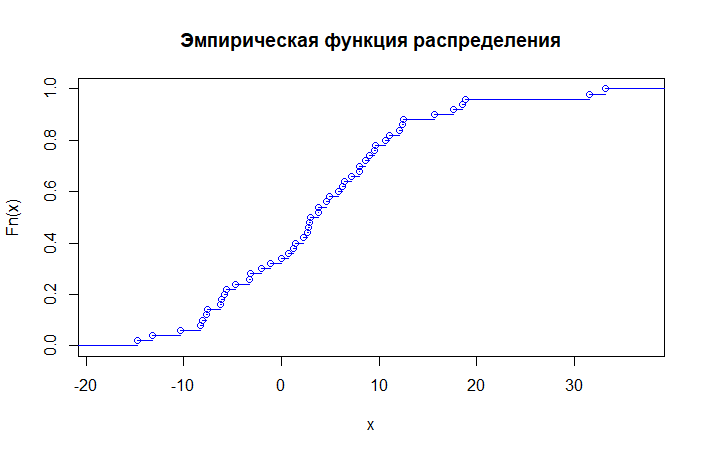
\includegraphics[scale=0.7]{Emp2.png}
		\caption{Эмпирическая функция распределения}
	\end{figure}
	\begin{figure}[h]
		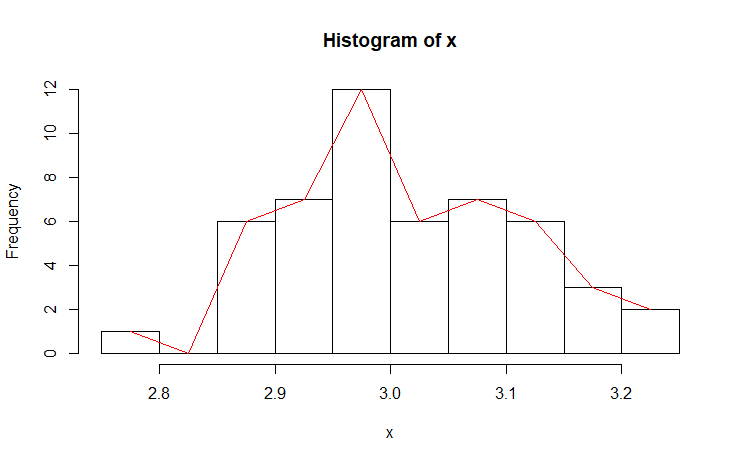
\includegraphics[scale=0.7]{Hist2.png}
		\caption{Гистограмма и полигон частот с шагом $h=0.05$}
	\end{figure}	
\end{proof}


\begin{problem}
	Вычислить выборочные аналоги следующих характеристик:
	\begin{itemize}
		\item математического ожидания
		\item дисперсии
		\item медианы
		\item ассиметрии
		\item эксцесса
		\item вероятности $P(X\in[c, d])$
	\end{itemize}
\end{problem}

\begin{proof}
	$ $	
	\begin{itemize}
		\item Математическое ожидание:
		\begin{equation}	
			\bar x_{\text{в}} = \cfrac1n\sum^{n}_{i=1}(x_i)=3.0116
		\end{equation}
		\item Дисперсия:
		\begin{equation}	
			D_{\text{в}} = \bar{x^2}-\bar{x}^2=\cfrac1n\sum\limits_{i=1}^n(x_i-\bar{x})^2=0.00970184
		\end{equation}
		\item Медиана:
		\begin{equation}
			Me = 2.993
		\end{equation}	
		\item Ассиметрия:
		\begin{equation}
			As = \cfrac{\mu_3^*}{\sigma^3} = 0.1669468
		\end{equation}
		\item Эксцесс:
		\begin{equation}
			Ex = \cfrac{\mu_4^*}{\sigma^4}-3 = -0.5054119
		\end{equation}
		\item Вероятность:
		\begin{equation}
			P(x \in [c, d]) = P(x \in [2.90, 3.06]) = F(3.06) - F(2.90) = 0.5 
		\end{equation}
	\end{itemize}			
\end{proof}


\begin{problem}
	В предположении, что исходные наблюдения являются выборкой из нормального распределения, построить оценку максимального правдоподобия параметров $(a, \sigma^2)$, и соответствующие оценки по методу моментов. Найти смещение оценок. 	
\end{problem}

\begin{proof}
	$ $
	
	Плотность нормального распределения:
	\begin{equation}
		f(x)=\cfrac{1}{\sigma\sqrt{2\pi}} \cdot \exp({-\cfrac{(x-a)^2}{2\sigma^2}})
	\end{equation}

	\begin{itemize}
		\item Метод максимального правдоподобия
		\begin{align}
			& \text{Функция правдоподобия:} \\
			& L(\vec{x}, a, \sigma^2)=\cfrac{1}{\sigma^n\sqrt{(2\pi)^n}} \cdot \exp({-\cfrac1{2\sigma^2}}\sum\limits_{i=1}^n(x_i-a)^2) \\
			& \text{Прологарифмируем:} \\
			& LL(\vec{x}, a, \sigma^2)=\cfrac{n}{2}log2\pi\sigma^2-\cfrac{1}{2\sigma^2}\sum\limits_{i=1}^n(x_i-a)^2 	
		\end{align}	
		$\left\lbrace
		\begin{gathered}
			\cfrac{\partial LL(\vec{x}, a, \sigma^2)}{\partial a}=\cfrac{1}{\sigma^2}\left(\sum\limits_{i=1}^nx_i-na\right)=0 \\
			\cfrac{\partial LL(\vec{x}, a, \sigma^2)}{\partial \sigma^2}=-\cfrac{n}{2\sigma^2}+\cfrac{1}{2(\sigma^2)^2}\sum\limits_{i=1}^n(x_i-a)^2=0 
		\end{gathered}	
		\right. \Rightarrow$	
		$\left\lbrace	
		\begin{gathered}	
			\hat{a}=\cfrac{\sum\limits_{i=1}^nx_i}{n}=\bar{x} \\
			\hat{\sigma^2}=\cfrac1n\sum\limits_{i=1}^n(x_i-\bar{x})^2=S^2 
		\end{gathered}
		\right.$ \\
		
		Найдем значения $\hat{a}=\bar{x}=3.0116$ - выборочное среднее и $\hat{\sigma^2}=S^2=0.00970184$ - выборочная дисперсия. \\
		\item Метод моментов
		\begin{align}
			& \text{В случае нормального распределения имеем }a_1'=\mathbb{E}(x)=a \text{ и } a_2'=\mathbb{E}(x^2)=\sigma^2+a^2 
		\end{align}	
		Уравнения моментов принимают вид:
		\begin{align}
			& \tilde{a}=\cfrac{1}{n}\sum\limits_{i=1}^nx_i=\bar{x}=3.0116 \\
			& \tilde{a^2}+\tilde{\sigma^2}=\cfrac1n\sum\limits_{i=1}^nx_i^2=\bar{x}^2
		\end{align}
		Откуда моментные оценки:
		\begin{align}
			& \tilde{a}=\bar{x}=3.0116 \\
			& \tilde{\sigma^2}=\bar{x}^2-\bar{x^2}=\cfrac{(\sum\limits_{i=1}^nx_i^2-\bar{x}\sum\limits_{i=1}^nx_i)}{n}=S^2=0.00970184
		\end{align}
	\end{itemize}
	Оценки являются несмещенными.
\end{proof}


\begin{problem}
	Построить доверительные интервалы уровня значимости $\alpha_2$ для параметров $(a, \sigma^2)$ 	
\end{problem}

\begin{proof}
	$ $
	
	Параметр $a$:
	\begin{align}
		& \sqrt{n-1}\left(\cfrac{\bar{x}-n}{s}\right)\sim S_{n-1} \\
		& x_{\alpha}:S_{n-1}(x_{\alpha})=1-\cfrac{\alpha_2}{2}
	\end{align}

	Тогда получаем:
	\begin{equation}
		P\left(-x_{\alpha}\leqslant\sqrt{n-1}\left(\cfrac{\bar{x}-n}{s}\right)\leqslant x_{\alpha}\right)=1-\alpha_2=P\left(\bar{x}-\cfrac{x_{\alpha}s}{\sqrt{n-1}}\leqslant a\leqslant\bar{x}+\cfrac{x_{\alpha}s}{\sqrt{n-1}}\right)
	\end{equation}
	ДИ уровня значимости $\alpha_2=0.20$ для $a$:
	\begin{equation}
		[2.9997; 3.0235]
	\end{equation}

	Параметр $\sigma^2$:
	\begin{equation}
		\cfrac{ns^2}{\sigma^2}\sim \chi^2_{n-1}
	\end{equation}

	Тогда выберем $x_{1\alpha}, x_{2\alpha}$ - квантили распределения $\chi^2_{n-1}$ уровня $\cfrac{\alpha_2}2$ и $1-\cfrac{\alpha_2}2$ соответственно, тогда $p\left(\cfrac{nS^2}{x_{1\alpha}}\leqslant \sigma^2 \leqslant \cfrac{nS^2}{x_{2\alpha}}\right)=1-\alpha_2$ \\
	ДИ уровня значимости $\alpha_2=0.20$ для $\sigma^2$: 
	\begin{align}
		[0.0078178; 0.0131728]
	\end{align}
\end{proof}


\begin{problem}
	С использованием теоремы Колмогорова построить критерий значимости проверки простой гипотезы согласия с нормальным распределением с параметрами $a_0, \sigma_0^2$. Проверить гипотезу на уровне значимости $\alpha_2$. Вычислить наибольшее значение уровня значимости, на котором нет оснований отвергнуть данную гипотезу.
\end{problem}

\begin{proof}
	$ $
	
	Простая гипотеза $H_0: a=a_0=2.60, \sigma^2=\sigma_0^2=0.10$ 
	
	Согласно теореме Колмогорова, при справедливости гипотезы:
	\begin{equation}
		\sqrt{n}sup|F_n(x)-F_0(x)|\rightarrow K(x)\text{, где $K(x)$ - функция Колмогорова}
	\end{equation}
	\begin{align}
		& K(C_{\alpha_2})=1-\alpha_2=1-0.2=0.8 \\
		& C_{\alpha_2}=C_{0.2}=1.0493 \\
		& H_0: X_1, ..., X_n\sim N(2.60, 0.10) 
	\end{align}
	С помощью $R$ вычислим:
	\begin{align}
		& sup|F_n(x)-F_0(x)| = 0.97573 \\
		& \sqrt{n}sup|F_n(x)-F_0(x)| = 6.658375 > 1.0493 \\
		& \text{Отвергаем гипотезу } H_0 \\
		& p-value = 2.2 \cdot 10^{-16} 
	\end{align}
	Наибольшее значение уровня значимости, на котором нет оснований отвергнуть гипотезу
\end{proof}


\begin{problem}
	Используя гистограмму частот, построить критерий значимости $\chi^2$ проверки простой гипотезы согласия с нормальным распределением с параметрами $(a_0, \sigma_0^2)$. Проверить гипотезу на уровне значимости $\alpha_2$. Вычислить наибольшее значение уровня значимости, на котором еще нет оснований отвергнуть данную гипотезу. 
\end{problem}

\begin{proof}
	$ $
	\begin{align}
		& H_0: X_1, ..., X_n\sim N(2.6, 0.1) \\
		& \sum\limits_{i=1}^k\cfrac{(m_i-m_i')^2}{m_i}\rightarrow\chi^2_{\text{кр}} \\
		& \chi^2_{\text{кр}} = \chi^2_4 = 5.988617 
	\end{align}
	Перестроим гистограмму частот, выбрав следующие точки: $(-Inf, 2.9, 2.97, 3.08, 3.15, Inf)$ 
	\begin{figure}[h]
		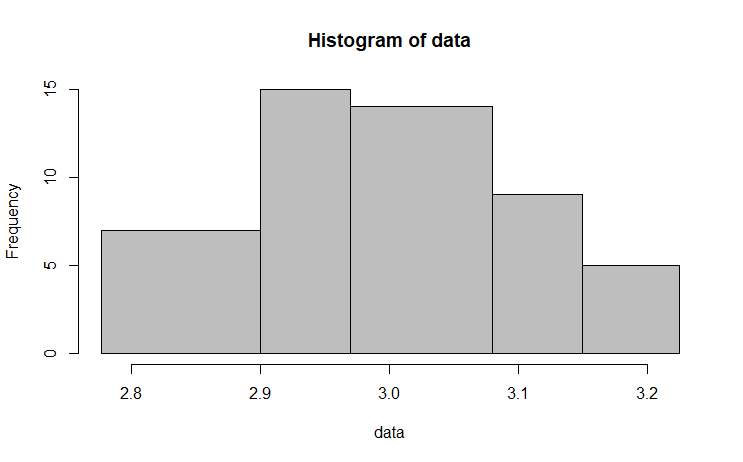
\includegraphics[scale=0.7]{Hist3.png}
	\end{figure} \\
	\begin{tabular}{|c|c|c|c|c|c|c|}
		\hline
		Интервал & $(-\infty; 2.9]$ & $(2.9; 2.97]$ & $(2.7; 3.08]$ & $(3.08; 3.15]$ & $(3.15; \infty)$ & $\sum$ \\ \hline 
		$m_i$ & $7$ & $15$ & $14$ & $9$ & $5$ & $50$ \\ \hline 
		$p_i$ & $0.9987$ & $0.0012$ & $0.0001$ & $\sim 0$ & $\sim 0$ & $1$ \\ \hline 
		$\cfrac{(m_i-m_i^{'})^2}{m_i^{'}}$ & $36$ & $3592$ & $36605$ & $2092090$ & $26330240$ & $\chi^2_{\text{набл}}$ \\
		\hline
	\end{tabular}
	\begin{align}
		\chi^2_{\text{набл}}&=28462569 \gg \chi^2_{\text{кр}}=5.988617 \\
		& P(\chi^2_{\text{набл}}>28462569) \rightarrow 0
	\end{align}
	Гипотеза отвергается, а точность чисел не позволяет вычислить наибольшее значение уровня значимости, на котором еще нет оснований отвергнуть гипотезу (оно крайне близко к 0).
\end{proof}


\newpage
\begin{problem}
	Построить критерий значимости $\chi^2$ проверки сложной гипотезы согласия с нормальным распределением. Проверить гипотезу на уровне значимости $\alpha_2$. Вычислить наибольшее значение уровня значимости, на котором еще нет оснований отвергнуть данную гипотезу. 
\end{problem}

\begin{proof}
	$ $
	\begin{align}
		& H_0: X_1, ..., X_n\sim N(a \sigma^2) \\
		& \sum\limits_{i=1}^k\cfrac{(m_i-np_i(a, \sigma^2))^2}{np_i(a, \sigma^2)}\rightarrow\chi^2_{\text{кр}} \\
	\end{align}
	Метод минимизации хи-квадрат: \\
	\begin{equation}
		\underset{a, \sigma^2}{argmin}\sum\limits_{i=1}^k\cfrac{(m_i-np_i(a, \sigma^2))^2}{np_i(a, \sigma^2)}\rightarrow\chi^2_{\text{кр}}
	\end{equation}
	Задача реализована в R с помощью скрипта: \\
	
	$\begin{gathered}	
		P <- function(a)\{ \hfill \\
		p <- 0 \hfill \\
		p[1] <- pnorm(2.9, a[1], a[2]) \hfill \\
		p[2] <- pnorm(2.97, a[1], a[2]) - sum(p) \hfill \\
		p[3] <- pnorm(3.08, a[1], a[2]) - sum(p) \hfill \\
		p[4] <- pnorm(3.15, a[1], a[2]) - sum(p) \hfill \\
		p[5] <- 1 - sum(p) \hfill \\
		p\} \hfill \\
		X2 <- function(a)\{g <- n*P(a); f <- (nu-g)^2/g; sum(f)\} \hfill \\
		nu <- c(7, 15, 14, 9, 5) \hfill \\
		a <- c(mean(data), sqrt(var(data))) \hfill \\
		XM <- nlm(X2, a)  \hfill \\
	\end{gathered}$	\\

	С помощью функции $nlm$ был найден минимум $\chi^2$:
	\begin{align}
		\chi^2_{\text{набл}}=3.928807, a&=3.0045, \sigma=0.1086 \\
		\chi^2_{\text{набл}} > &\chi^2_{\text{кр}}=3.218876 
	\end{align}
	Сложная гипотеза согласия с нормальным распределением отвергается.
	\begin{equation}
		P(x > 3.928807) = 0.1402395
	\end{equation}
	Гипотеза может быть принята, если уровень значимости 
	\begin{equation}
		\alpha\leqslant 0.1402395
	\end{equation}
\end{proof}


\begin{problem}
	Построить наиболее мощный критерий проверки простой гипотезы о нормальности с параметром $(a, \sigma^2)=(a_0, \sigma_0^2)$ при альтернативе нормальности с параметром $(a, \sigma^2)=(a_1, \sigma_1^2)$. Проверить гипотезу на уровне значимости $\alpha_2$. Что получится, если поменять местами основную и альтернативную гипотезы?
\end{problem}

\begin{proof}
	$ $
	
	Отношение правдоподобия ($\sigma_0 = \sigma_1$):
	\begin{multline}
		l(x)=\cfrac{L(x, a_1, \sigma_1^2)}{L(x, a_0, \sigma_0^2)}=\cfrac{\sigma_0^n}{\sigma_1^n}\exp\left(\cfrac{1}{2\sigma_0^2}\left(\sum\limits_{i=1}^n(x_i-a_0)^2-\sum\limits_{i=1}^n(x_i-a_1)^2\right)\right)=\\=\exp\left(\cfrac{1}{2\sigma_0^2}\sum\limits_{i=1}^n-2x_ia_0+a_0^2+2x_ia_1-a_1^2\right)
	\end{multline}
	Логарифмируем:
	\begin{equation}
		\exp\left(\cfrac{1}{2\sigma_0^2}\sum\limits_{i=1}^n-2x_ia_0+a_0^2+2x_ia_1-a_1^2\right)>c\rightarrow \cfrac{1}{2\sigma_0^2}\sum\limits_{i=1}^n(a_0^2-a_1^2)+2x_i(a_1-a_0)>log c
	\end{equation}
	Отсюда:
	\begin{equation}
		\cfrac{n(a_0^2-a_1^2)}{2\sigma_0^2}+\cfrac{a_1-a_0}{\sigma_0^2}\sum\limits_{i=1}^nx_i>log c
	\end{equation}
	Подставив известные $n=50, \sigma_0=0.10, a_0=2.60, a_1=3.00$ получаем:
	\begin{equation}
		-5600+40\sum\limits_{i=1}^nx_i>logc\rightarrow\sum\limits_{i=1}^nx_i>\cfrac{logc+5600}{40}=c^* 
	\end{equation} 
	Тогда критерий примет вид: \\
	
	$\phi(x)=\left\{
	\begin{gathered}
		1, \sum\limits_{i=1}^nx_i>c^* \\
		p, \sum\limits_{i=1}^nx_i=c^* \\
		0, \sum\limits_{i=1}^nx_i<c^*
	\end{gathered}
	\right.$ \\
	
	С помощью R определим $c^*$ и получим: \\
	
	$\phi(x)=\left\{
	\begin{gathered}
		1, \sum\limits_{i=1}^nx_i>129 \\
		p, \sum\limits_{i=1}^nx_i=129 \\
		0, \sum\limits_{i=1}^nx_i<129
	\end{gathered}
	\right.$ \\
	
	В нашем случае $\sum\limits_{i=1}^nx_i=150>129$, поэтому принимается основная гипотеза о нормальности с параметром $(a_0, \sigma_0^2)$. 
	
	Если поменять местами основную и альтернативную гипотезы, то будет принята альтернативная гипотеза о нормальности с параметром $(a_1, \sigma_1^2)$.
\end{proof}


\begin{problem}
	В пунктах (c) - (g) заменить семейство нормальных распределений на двухпараметрическое семейство распределений Лапласа.
\end{problem}

\begin{proof}
	$ $
	
	Плотность распределения Лапласа: 
	\begin{equation}
		f(x)=\cfrac1{\sqrt{2}\sigma}\exp(-\cfrac{\sqrt{2}}{\sigma}|x-a|)
	\end{equation}
\end{proof}


\begin{problem}
	В предположении, что исходные наблюдения являются выборкой из распределения семейства Лапласа, построить оценку максимального правдоподобия параметров $(a, \sigma^2)$, и соответствующие оценки по методу моментов. Найти смещение оценок. 
\end{problem}

\newpage
\begin{proof}
	$ $
	
	\begin{itemize}
		\item Метод максимального правдоподобия
		\begin{align}
			l(\vec{x}, a, \sigma^2)=\cfrac{1}{\sigma^n2^{n/2}}\exp(-\cfrac{\sqrt{2}}{\sigma}&\sum\limits_{i=1}^n|x_i-a|) \\
			ll(\vec{x}, a, \sigma^2) = -nlog(\sigma)-\cfrac{n}{2}log(2)-\cfrac{\sqrt{2}}{\sigma}&\sum\limits_{i=1}^n|x_i-a| = \\
			= -nlog(\sigma)-\cfrac{n}{2}log(2)-\cfrac{\sqrt{2}}{\sigma}\sum\limits_{i=1}^k(a-x_{(i)})-\cfrac{\sqrt{2}}{\sigma}&\sum\limits_{i=k+1}^n(x_{(i)}-a) = \\
			= -nlog(\sigma)-\cfrac{n}{2}log(2)-\cfrac{\sqrt{2}}{\sigma}ka+\cfrac{\sqrt{2}}{\sigma}\sum\limits_{i=1}^kx_{(i)}-\cfrac{\sqrt{2}}{\sigma}&\sum\limits_{i=k+1}^nx_{(i)}+\cfrac{\sqrt{2}}{\sigma}(n-k-1)a = \\
			= -nlog(\sigma)-\cfrac{n}{2}log(2)+\cfrac{\sqrt{2}}{\sigma}\sum\limits_{i=1}^kx_{(i)}-\cfrac{\sqrt{2}}{\sigma}\sum\limits_{i=k+1}^nx_{(i)}+&\cfrac{\sqrt{2}}{\sigma}(n-k-1)a+\cfrac{\sqrt{2}}{\sigma}(n-2k-1)a
		\end{align}
		\begin{align}
			& \cfrac{\partial ll(\vec{x}, a, \sigma^2)}{\partial a}=\cfrac{\sqrt{2}}{\sigma}(n-2k-1) \\
			& \cfrac{\sqrt{2}}{\tilde{\sigma}}(n-2k-1)=0 \\
			& k = \cfrac{n-1}{2} - \text{выборочная медиана} \\
			& \tilde{a}\in (x_{(\frac{n}{2})}, x_{(\frac{n}{2}+1)})=(x_{(25)}, x_{(26)})=(2.987, 2.998)=2.9925 \\
			& \cfrac{\partial ll(\vec{x}, a, \sigma^2)}{\partial \sigma}=-\cfrac{n}{\sigma}+\cfrac{\sqrt{2}}{\sigma^2}\sum\limits_{i=1}^n|x_i-a| \\
			& -\cfrac{n}{\tilde{\sigma}}+\cfrac{\sqrt{2}}{\tilde{\sigma}^2}\sum\limits_{i=1}^n|x_i-a|=0 \\
			& \tilde{\sigma}=\cfrac{1}{n}\sum\limits_{i=1}^n|x_i-\tilde{a}|
		\end{align}
		Оценка максимального правдоподобия: \\
		\begin{equation}
			(\tilde{a}, \tilde{\sigma}) = (2.9925, 0.006599938) 
		\end{equation}
		\newpage
		\item Метод моментов
		\begin{align}
			& \mathbb{E}(x)=a\rightarrow=\hat{a}=\bar{x}=3.0116 \\
			& \mathbb{D}(x)=\cfrac{2}{\frac{2}{\sigma^2}}=\sigma^2\rightarrow\hat{\sigma^2}=s^2=0.00970184 \\
			& (\hat{a}, \hat{\sigma^2})=(\tilde{a}, \tilde{\sigma^2})=(3.0116, 0.00970184)
		\end{align}
	\end{itemize}
	\begin{align}
		& \mathbb{E}(\hat{a})=\mathbb{E}(\bar{x})=a\rightarrow\text{несмещенная оценка} \\
		& \mathbb{E}(\hat{\sigma^2})=\mathbb{E}(s^2)=\frac{n-1}{n}\sigma^2\rightarrow\mathbb{E}(\hat{\sigma^2})-\sigma^2=\frac{n-1}{n}\sigma^2-\sigma^2=-\frac{\sigma^2}{n}\rightarrow\text{смещенная оценка}
	\end{align}
\end{proof}


\begin{problem}
	Построить доверительные интервалы уровня значимости $\alpha_2$ для параметров $(a, \sigma^2)$ 	
\end{problem}

\begin{proof}
	$ $
	
	Параметр $a$:
	\begin{equation}
		\cfrac{\sum_{i=1}^nx_i-na}{\sqrt{n\sigma^2}}\rightarrow N(0, 1); \cfrac{\sum_{i=1}^nx_i-na}{\sqrt{ns^2}}\rightarrow N(0, 1)
	\end{equation}

	Выберем $t_{\gamma}: \phi(t_{\gamma})=1-\cfrac{\alpha_2}2\Rightarrow t_{\gamma}=1.281552$ \\
	\begin{equation}
		P\left(-t_{\gamma} \leqslant \cfrac{\sqrt{n}(\bar{x}-a)}{s} \leqslant t_{\gamma}\right)=1-\alpha_2=P\left(\bar{x}-\cfrac{t_{\gamma} s}{\sqrt{n}}\leqslant x \leqslant \bar{x}+\cfrac{t_{\gamma} s}{\sqrt{n}}\right)
	\end{equation}

	Отсюда асимптотический ДИ уровня значимости 0.2:
	\begin{equation}
		[2.993748, 3.029452]
	\end{equation}

	Параметр $\sigma^2$:
	\begin{equation}
		\sqrt{n}(\tilde{\sigma}-\sigma)\sim N(0, \cfrac{\sigma^2}{2})
	\end{equation}
	\begin{equation}	
		\cfrac{\sqrt{2n}}{\cfrac{\sqrt{2}}{n}\sum_{i=1}^n|x_i-\tilde{a}|}\left(\cfrac{\sqrt{2}}{n}\sum_{i=1}^n|x_i-\tilde{a}|-\sigma\right)\sim N(0, 1)
	\end{equation}
	
	Найдем ДИ: \\
	\begin{align}
		& P\left(-t_{\gamma} \leqslant \cfrac{\sqrt{2n}}{\cfrac{\sqrt{2}}{n}\sum_{i=1}^n|x_i-\tilde{a}|}\left(\cfrac{\sqrt{2}}{n}\sum_{i=1}^n|x_i-\tilde{a}|-\sigma\right) \leqslant t_{\gamma}\right) = 1-\alpha_2 = \\
		& = P\left(\cfrac{\sqrt{2}}{n}\sum_{i=1}^n|x_i-\tilde{a}|-\cfrac{t_{\gamma}\sum_{i=1}^n|x_i-\tilde{a}|}{n^{\frac32}} \leqslant \sigma^2 \leqslant \cfrac{\sqrt{2}}{n}\sum_{i=1}^n|x_i-\tilde{a}|+\cfrac{t_{\gamma}\sum_{i=1}^n|x_i-\tilde{a}|}{n^{\frac32}} \right)
	\end{align}

	Вычислим ДИ:
	\begin{equation}
		[0.00903340, 0.01679993]
	\end{equation}
\end{proof}


\begin{problem}
	С использованием теоремы Колмогорова построить критерий значимости проверки простой гипотезы согласия с распределением из семейства Лапласса с параметрами $a_0, \sigma_0^2$. Проверить гипотезу на уровне значимости $\alpha_2$. Вычислить наибольшее значение уровня значимости, на котором нет оснований отвергнуть данную гипотезу.
\end{problem}

\begin{proof}
	$ $
	
	Простая гипотеза $H_0: a=a_0=2.60, \sigma^2=\sigma_0^2=0.10$ 
	
	Согласно теореме Колмогорова, при справедливости гипотезы:
	\begin{equation}
		\sqrt{n}sup|F_n(x)-F_0(x)|\rightarrow K(x)\text{, где $K(x)$ - функция Колмогорова}
	\end{equation}
	\begin{align}
		& K(C_{\alpha_2})=1-\alpha_2=1-0.2=0.8 \\
		& C_{\alpha_2}=C_{0.2}=1.0493 \\
		& H_0: X_1, ..., X_n\sim Laplace(2.60, 0.10) 
	\end{align}
	С помощью $R$ вычислим:
	\begin{align}
		& sup|F_n(x)-F_0(x)| = 0.9390869 \\
		& \sqrt{n}sup|F_n(x)-F_0(x)| = 6.640347 > 1.0493 \\
		& \text{Отвергаем гипотезу } H_0 \\
		& p-value = 2.2 \cdot 10^{-16} 
	\end{align}
	Наибольшее значение уровня значимости, на котором нет оснований отвергнуть гипотезу
\end{proof}


\begin{problem}
	Используя гистограмму частот, построить критерий значимости $\chi^2$ проверки простой гипотезы согласия с распределением из семейства Лапласса с параметрами $(a_0, \sigma_0^2)$. Проверить гипотезу на уровне значимости $\alpha_2$. Вычислить наибольшее значение уровня значимости, на котором еще нет оснований отвергнуть данную гипотезу. 
\end{problem}

\begin{proof}
	$ $
	\begin{align}
		& H_0: X_1, ..., X_n\sim Laplace(2.6, 0.1) \\
		& \sum\limits_{i=1}^k\cfrac{(m_i-m_i')^2}{m_i}\rightarrow\chi^2_{\text{кр}} \\
		& \chi^2_{\text{кр}} = \chi^2_4 = 5.988617 
	\end{align}
	Перестроим гистограмму частот, выбрав следующие точки: $(-Inf, 2.9, 2.97, 3.08, 3.15, Inf)$ 
	\begin{figure}[h]
		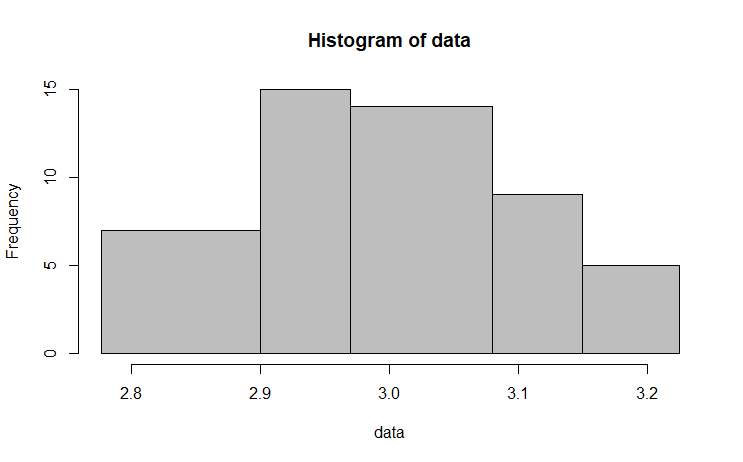
\includegraphics[scale=0.6]{Hist3.png}
	\end{figure} \\
	\begin{tabular}{|c|c|c|c|c|c|c|}
		\hline
		Интервал & $(-\infty; 2.9]$ & $(2.9; 2.97]$ & $(2.7; 3.08]$ & $(3.08; 3.15]$ & $(3.15; \infty)$ & $\sum$ \\ \hline 
		$m_i$ & $7$ & $15$ & $14$ & $9$ & $5$ & $50$ \\ \hline 
		$p_i$ & $0.9928152020$ & $0.0045149597$ & $0.0021063547$ & $0.0003540957$ & $0.0002093880$ & $1$ \\ \hline 
		$\cfrac{(m_i-m_i^{'})^2}{m_i^{'}}$ & $36.62785$ & $966.91238$ & $1833.14041$ & $4557.05246$ & $2377.92240$ & $\chi^2_{\text{набл}}$ \\
		\hline
	\end{tabular}
	\begin{align}
		\chi^2_{\text{набл}}&=9771.655 > \chi^2_{\text{кр}}=5.988617 \\
		& P(\chi^2_{\text{набл}}>9771.655) \rightarrow 0
	\end{align}
	Гипотеза отвергается, а точность чисел не позволяет вычислить наибольшее значение уровня значимости, на котором еще нет оснований отвергнуть гипотезу (оно крайне близко к 0).
\end{proof}


\newpage
\begin{problem}
	Построить критерий значимости $\chi^2$ проверки сложной гипотезы согласия с распределением из семейства Лапласса. Проверить гипотезу на уровне значимости $\alpha_2$. Вычислить наибольшее значение уровня значимости, на котором еще нет оснований отвергнуть данную гипотезу. 
\end{problem}

\begin{proof}
	$ $
	\begin{align}
		& H_0: X_1, ..., X_n\sim Laplace(a \sigma^2) \\
		& \sum\limits_{i=1}^k\cfrac{(m_i-np_i(a, \sigma^2))^2}{np_i(a, \sigma^2)}\rightarrow\chi^2_{\text{кр}} \\
	\end{align}
	Метод минимизации хи-квадрат: \\
	\begin{equation}
		\underset{a, \sigma^2}{argmin}\sum\limits_{i=1}^k\cfrac{(m_i-np_i(a, \sigma^2))^2}{np_i(a, \sigma^2)}\rightarrow\chi^2_{\text{кр}}
	\end{equation}
	С помощью функции $nlm$ был найден минимум $\chi^2$:
	\begin{align}
		\chi^2_{\text{набл}}=7.530788, a&=2.9898297, \sigma=0.1375121 \\
		\chi^2_{\text{набл}} > &\chi^2_{\text{кр}}=3.218876 
	\end{align}
	Сложная гипотеза согласия с нормальным распределением отвергается.
	\begin{equation}
		P(x > 7.530788) = 0.02315849
	\end{equation}
	Гипотеза может быть принята, если уровень значимости 
	\begin{equation}
		\alpha\leqslant 0.02315849
	\end{equation}
\end{proof}